\chapter{Realizace a testování}

Praktickým výstupem práce je samotná realizace a otestování zařízení bez solárního napájení. Vybrané komponenty byly umístěny do plastové konstrukční krabičky, která byla upravena s ohledem na rozmístění jednotlivých komponent.

Na předním straně krabičky je čočka PIR senzoru, infračervená LED dioda a kamera. Na vrchní straně se nachází anténa pro GSM modul. 

Na pravém boku je 2.1 mm napájecí konektor. Je možné připojit akumulátor nebo stejnosměrný napájecí zdroj. Tolerované napájecí napětí je 8--20 V.

Dále se zde nachází tlačítko pro zapnutí čí vypnutí zařízení. Vypínání je řešeno softwarově, takže po stisku nedochází k úplnému vypnutí zařízení ale pouze k přepnutí do režimu halt. 


\begin{figure}[!h]
  \begin{center}
    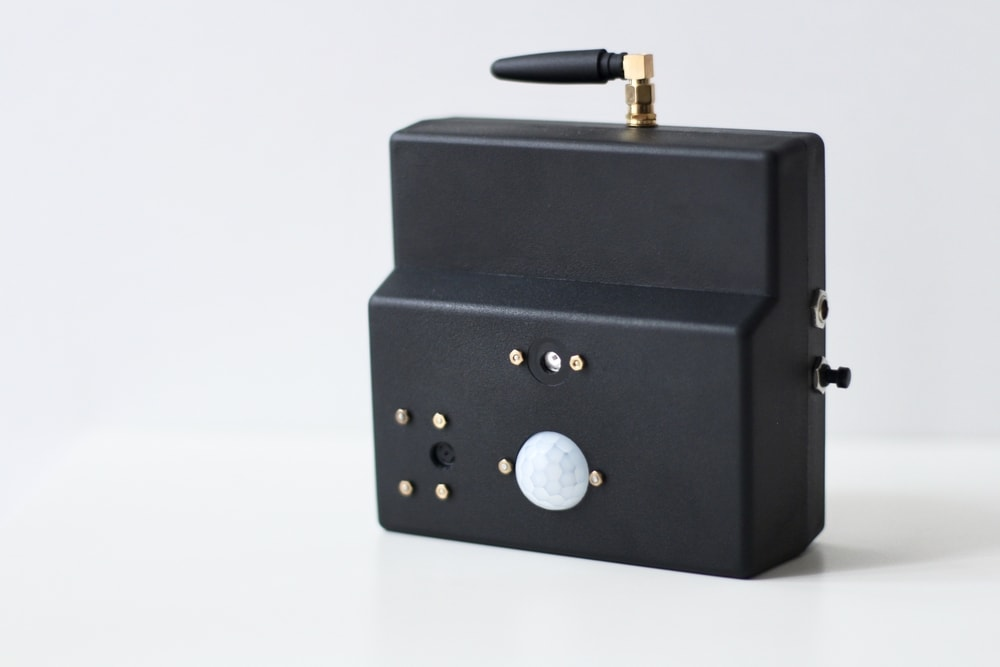
\includegraphics[scale=0.4]{obrazky/kamera.jpg}
  \end{center}
  \caption{Realizace kamerového zabezpečovacího systému}
\end{figure}


\begin{figure}[!h]
  \begin{center}
    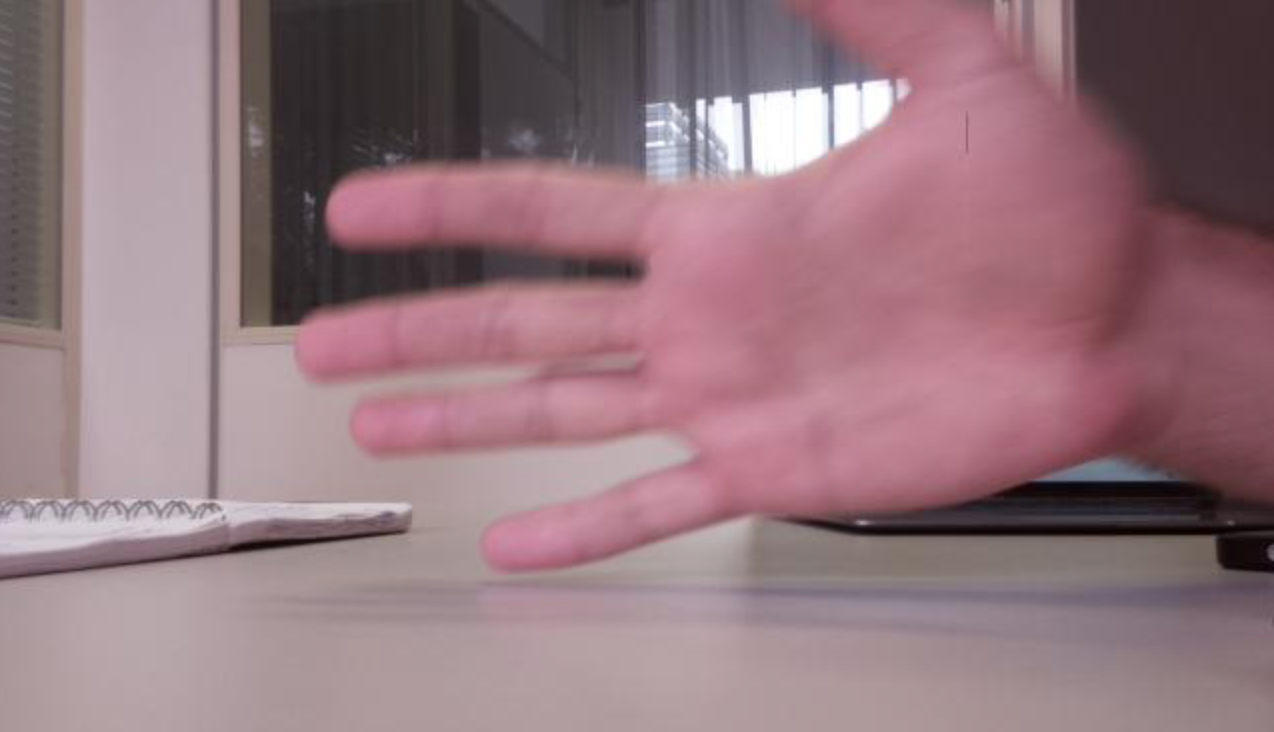
\includegraphics[scale=0.5]{obrazky/ukazka.png}
  \end{center}
  \caption{Ukázka denní fotografie pořízené kamerou}
\end{figure}

\begin{figure}[!h]
  \begin{center}
    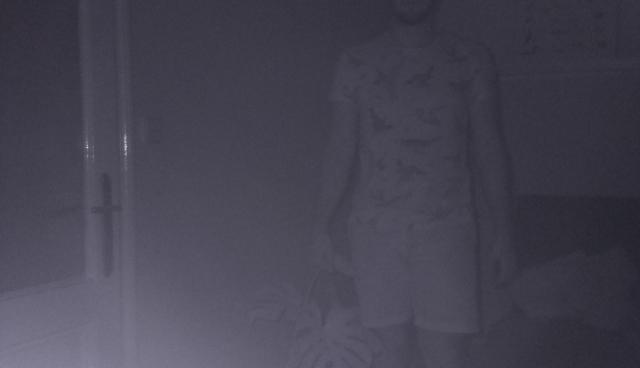
\includegraphics[scale=0.5]{obrazky/night_photo.jpg}
  \end{center}
  \caption{Ukázka noční fotografie pořízené kamerou s IR přísvitem}
\end{figure}

\clearpage

\section{Publikace aplikace}
Zdrojové kódy aplikace jsou spolu s dokumentací zveřejněny na serveru GitHub.

\href{www.github.com/marekvi95/bakalarka}{\textbf{www.github.com/marekvi95/bakalarka}}

\dirtree{%
 .1 /.
 .2 rpicameramon\DTcomment{hlavní modul}.
 .3 init.
 .3 motion.
 .3 config.
 .3 filemanipulation.
 .3 telemetry.
 .2 google\DTcomment{skripty na google API}.
 .3 scripts.
 .4 main.
 .4 index.
 .2 init\DTcomment{spouštění po startu}.
 .3 listen-shutdown.
 .2 docs\DTcomment{dokumentace aplikace}.
 .2 gsm\DTcomment{komunikace s gsm modulem}.
 }


\subsection*{Dokumentace}
K dokumentaci aplikace je použit generátor dokumentace Sphinx. Dokumentace ve zdrojovém kódu je realizována pomocí konvence Google docstring.

Dokumentace je napsaná v anglickém jazyce.


\chapter{Závěr}

V práci byla prozkoumána možná řešení a byl rámcově zpracován návrh kamerového zabezpečovacího systému založeného na minipočítači Raspberry Pi. 

V teoretické části práce byly vybrány hardwarové komponenty vhodné pro aplikaci na detekci pohybu s ohledem na co nejnižší spotřebu elektrické energie. Při výběru softwaru byl dáván důraz na jeho aktuálnost, otevřenost a rozšířitelnost. Z těchto důvodů byl pro práci vybrán jako hlavní programovací jazyk Python.  

V druhé kapitole je popsán návrh samotné aplikace pro detekci z obrazu a též za pomocí PIR senzoru. Důraz je kladen na konfigurovatelnost aplikace.

Třetí kapitola se věnuje návrhu napájení jednotlivých komponent pomocí solárního panelu a akumulátoru.

Poslední kapitola se věnuje realizaci zařízení a testování funkčnosti.

\section{Možná vylepšení}
Praktická realizace zařízení ukázala nedostatky při použití minipočítače Raspberry Pi. Vzhledem k požadavku na bateriové napájení se jako vhodnější jeví použití mikrokontroléru s podporou uspávání, které by pomohlo ušetřit energii v době neaktivity zařízení. Další možností je například implementace detektoru pohybu na FPGA. Tato možnost by mohla přinést nižší nároky na napájení a také rychlejší a spolehlivější zpracování obrazu.

Za zvážení by také stálo použití kamery s lepším objektivem, který by umožnil pořizovat kvalitnější fotografie.

Pro připojení k sítí Internet by bylo vhodnější použít modul podporující sítě čtvrté generace. Nástupce modelu SIM800 je SIM7100 od firmy Simcomm, který podporuje i nový standard úzkopásmového LTE NB IoT. V takovém případě by nebylo nutné provádět úpravy ve stávajícím softwaru.

Co se týká aplikace pro detekci, tak jako možné vylepšení se nabízí lokalizace a klasifikace objektu, tak aby bylo možné rozeznávat, zda se jedná o člověka nebo o zvíře. Případná další vylepšení by mohla přinést aplikace neuronových sítí.





